
\section{Функции, заданные неявно}
\subsection{Основные понятия}
\begin{equation} \label{eq:1}\
f(x,y)=0; 
\end{equation}
$D_{f}=\{(x,y)\in\mathbf{E}^2: f(x,y)=0 \} $  - график уравнения \ref{eq:1}. $D_f \leftrightarrow Ox$


\begin{minipage}{100mm}
	\subsubsection{Примеры}
	\begin{enumerate}
		\item $x^2+y^2-1=0$ \\
		$f_x=2x; \; f_y=2y$ \\
		Точку (0,1), например, нельзя рассматривать как y=f(x), но можно как x=f(y)
		\item$ (x-y)(x+y-1)=0$ \\
		$f_x=(x+y-1)+(x-y); \;\; f_y=-(x+y-1)+(x-y)$
		$(\frac 1 2;\frac 1 2)$ - особая точка, где обе 0.  Ни по Ox, ни по Oy нет биекции.
	\end{enumerate}
\end{minipage}
\begin{minipage}{70mm}
	\begin{figure}[H]
		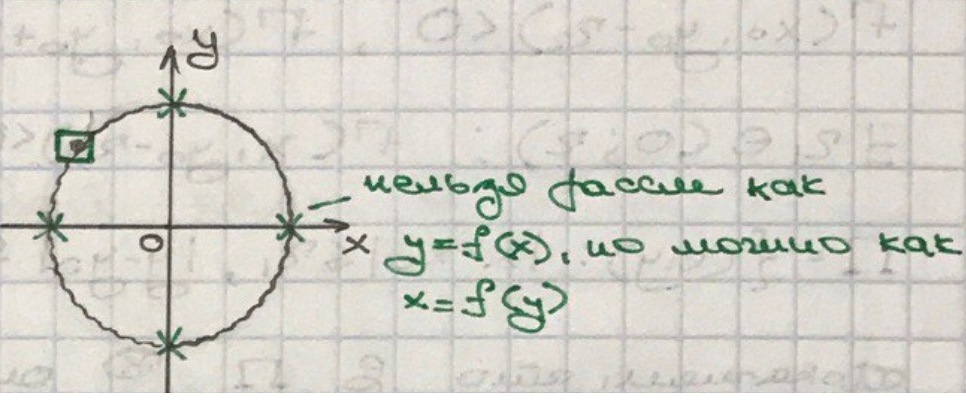
\includegraphics[width=50mm]{lect1pic1}
		\\
		\\
		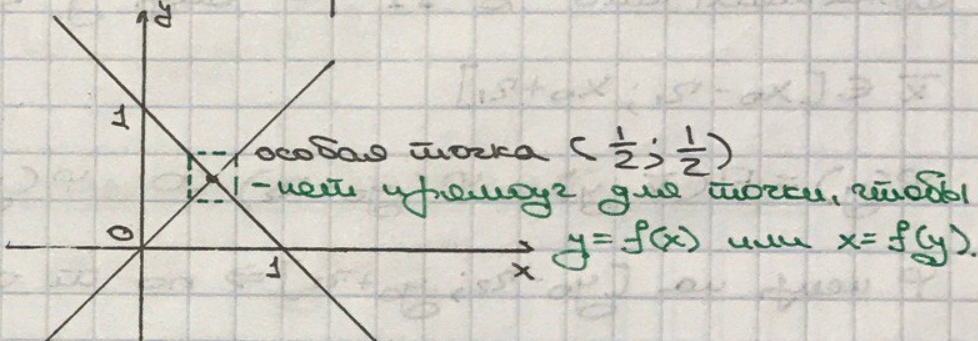
\includegraphics[width=50mm]{lect1pic2}
		\\
	\end{figure}
\end{minipage}

\subsection{Теорема о неявно заданной функции}
Достаточное условие, при котором уравнение \ref{eq:1} локально определеяет y как $f(x)$ и y обладает некоторыми дифф. свойствами.

\begin{theorem}
	Если \begin{enumerate}
		\item $f(x_0,y_0)=0$ \label{enum:1}
		\item в некоторой $u(x_0,y_0)$ функция f обладает непрерывной частной производной\label{enum:2}
		\item $f_y(x_0,y_0)\ne0,$ \label{enum:3}
	\end{enumerate}
То $\exists \Pi=\{(x,y): |x-x_0|\leq r_1, |y-y_0|\leq r_2\} \in U(x_0,y_0)$ в пределах которого уравнение \ref{eq:1} определяет y как функцию переменной x $(y=f(x))$, которая непрерывно дифференцируема на $(x_0-r_1, x_0+r_1)$ и $y'=-\frac{f_x(x,y)}{f_y(x,y)}\left.\right|_{y=f(x)}$
\end{theorem}
\begin{proof}
\textbf{I. Существование неявно заданной функции}\\
	$\ref{enum:3}\Rightarrow$  Пусть $f_y(x_0,y_0)>0 \; \rightarrow_{(2)} \exists \Pi_1= \{(x,y): |x-x_0|\leq r, |y-y_0|\leq r_2\}\in U(x_0,y_0)$ такой, что $\forall (x.y)\in \Pi_1 \Rightarrow f_y(x,y)>0$ \\
	$\psi(y)=f(x_0,y), \; \psi(y_0)=0, \; \psi $- возрастает на $[y_0-r_2, y_0+r_2]$\\
	$\psi'(y)=f_y(x_0,y)>0, \; \forall y\in [y_0-r_2, y_0+r_2] \Rightarrow \psi(y_0-r_2)<0, \psi(y_0+r_2)>0$\\
	$f(x_0, y_0 - r_2)<0, \; f(x_0,y_0+r_2)>0\\
	\exists r_1\in(0,r): \; f(x,y_0-r_2)<0, f(x,y_0+r_2)>0, \forall x\in[x_0-r, x_0+r] \\ \Pi=\{(x,y): |x-x_0|\leq r_1, |y-y_0|\leq r_2\}\in U(x_0,y_0)$\\
	Покажем, что в $\Pi \ref{eq:1}$ определяет $y$ как функцию от $x$\\
	$\overline{x}\in [x_0-r_1, x_0+r_1]\\
	\phi(y)=f(\overline{x},y), \; \phi(y_0-r_2)<0,\; \phi(y_0+r_2)>0$\\
	$\phi(y)$ непрерывна на $[y_0-r_2;y_0+r_2]\Rightarrow$ по теореме о промежуточном значении $\exists \overline{y} \in (y_0-r_2;y_0+r_2): \phi(\overline{y})=0 $ и эта точна единственная.\\
	$\phi'(y)=f_y(\overline{x},y)>0$ в $\Pi_1\subset\Pi \\
	f(\overline{x},\overline{y})=0 \;\; y=f(x)$\\
\textbf{II.}\\	
	$\Pi_1= \{(x,y): |x-x_0|\leq r_1, |y-y_0|\leq r_2\}$\\
	$(x_0,y_0)\in \Pi, \; f(x_0,y_0)=0, \;(x_0+\Delta x, y_0 + \Delta y)\in \Pi$ и $f(x_0+\Delta x,y_0+\Delta y)=0; \\
	\Delta  f=f(x_0+\Delta x,y_0+\Delta y) - f(x_0, y_0)=0;\\
	\Delta  f=f(x_0+\Delta x,y_0+\Delta y) -f(x_0,y_0+\Delta y)+f(x_0,y_0+\Delta y)-  f(x_0, y_0)=0;\\
	\exists \Theta_1, \Theta_2: 0<\Theta_I<1: \Delta  f=f_x(x_0+\Theta_1\Delta x,y_0+\Delta y)\Delta x +f_y(x_0+\Delta x,y_0+\Theta_2\Delta y)\Delta y=0;$\\
	$$\Delta y=- \frac{f_x(x_0+\Theta_1\Delta x,y_0+\Delta y)}{f_y(x_0+\Delta x,y_0+\Theta_2\Delta y)}\Delta x \Rightarrow |\Delta y|\leq \frac{M}{m}|\Delta x| $$
	$\Rightarrow$ при $\Delta x\rightarrow0, \Delta y \rightarrow 0\;\; f_y$ непрерывно в $\Pi$ - компакт  $\Rightarrow \exists m>0: f_y(x,y)\geq m; \;\exists M>0: |f_y(x,y)|\leq M  $ на  $\Pi$ 
	$$\frac{\Delta y}{\Delta x}=-\frac{f_x(x_0+\Theta_1\Delta x, y_0+\Delta y )}{f_y(x_0,y_0+\Theta_2\Delta y)}; \;\;
	f'(x_0)=-\frac{f_x(x_0,f(x_0))}{f_y(x_0,f(x_))};\;\; y_0=-f(x_0);$$
	В силу произвольности $(x_0,y_0)$ производная существует на всем $(x_0-r_1, x_0+r_1)$
\end{proof}
\textbf{Замечание}\\
Теорема остается справедливой, если в $f(x,y)=0, \; x=(x_1,x_2,\dots, x_m)$\\
$\Pi=\{(x_1,x_2,\dots, x_m,y): |x_i-x^0_i|_{i=\overline{1,m}}\leq r_i, |y-y_0|\leq \rho \}$

\subsection{Неявные функции, определяемые системой уравнений}
$$\left\{
\begin{aligned}\label{al:1}
f_1(x_1, \dots, x_n, y_1, \dots y_n )=0\\
f_2(x_1, \dots, x_n, y_1, \dots y_n )=0\\
\dots \\
f_n(x_1, \dots, x_n, y_1, \dots y_n )=0\\
\end{aligned}
\right.
$$\\
$x^0\in\mathbb{E}^m, y^0 \in \mathbb{E}^n; \; 
 \Pi(x^0)=\{x\in \mathbb{E}^m: |x_i-x_i^0|\leq r_i, i=\overline{1,m}\}$ \\
$\Pi(y^0)=\{y\in \mathbb{E}^n: |y_i-y_i^0|\leq \rho_i, i=\overline{1,n}\}$ \\
$\Pi=\Pi(x^0)\times \Pi(y_0)=\{(x,y)\in \mathbb{E}^n+m: x\in\Pi(x^0), y\in \Pi(y^0)\}$\\
Система  определяет в $\Pi\; y_1,\dots,y_n$ как неявные функции переменных $x_1, \dots x_m$, если $\forall x \in \Pi(x^0)$ ставится в соответствие такое $y\in \Pi(x^0),$ что $f_i(x,y)=0, \; i\in\overline{1,n}$ 
\begin{theorem}
	Пусть 
	\begin{enumerate}
		\item $f_i(x^0,y^0)=0, \;i\in\overline{1,n}$
		\item Функции $f_i, i\in\overline{1,n}$ обладают в некоторой окрестности $U(x^0,y^0) $ непрерывностью частных проихводных по переменным $x_j, j\in\overline{1,m}$ и $y_i, i\in\overline{1,n}$ 
		\item 
		$\begin{vmatrix}
			\frac{\partial f_1}{\partial y_1} & \dots & \frac{\partial f_1}{\partial y_n}	 \\
			 & \dots & 	 \\
			\frac{\partial f_n}{\partial y_1}& \dots & \frac{\partial f_n}{\partial y_n}
		\end{vmatrix}(x^0,y^0)\ne 0$
	\end{enumerate}
	Тогда $\exists \Pi=\Pi(x^0)\times |pi(y^0) \in U$, в пределах которого система определяет переменные $y_1,\dots,y_n$ как неявно заданные функции переменных $x_1,\dots,x_m$ и эти функции $y_i=f_i(x)$ обладают непрерывными частными производными в $\Pi(x^0)$ и $y^0_i=f'^i(x^0), \overline{1,n}$
\end{theorem}



